\chapter{State of the art}
%\minitoc


%%%%%%%%%%%%%%%%%%%%%%%%%%%%%%%%%%%%%%%%%%%%%%%%%%%%%
\section{Facial Recognition}
The challenge of face recognition can be formulated as followed :  with one or several images of a face, the goal would be to find or check the identity of a person by comparing his face to all the face images stored in a database. By the way this skill remains the most acceptable because it more suits with what human beings use in visual interaction; and compared to other methods, the face recognition seems more advantageous, in fact it is a non-intrusive method, in other words it does not require the cooperation of the subject, and a moreover the sensors used are cheaper.


\subsection{Facial recognition process}
Any facial recognition process must take into consideration several factors that contribute to the complexity of its task, because a face is a dynamic entity which constantly changes under the influence of several factors. A facial recognition system is generally  divided into the following steps (see the figure):

\begin{figure}[bth]%[!ht]
\begin{center}
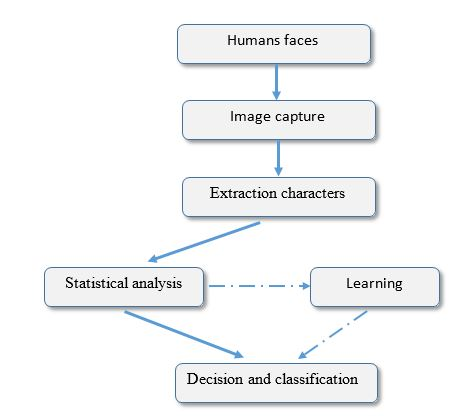
\includegraphics[scale=0.75]{fr_process}%[height=70mm,width=70mm]
\caption{\textbf{Facial recognition system process}}%
%\url {http://www.google.fr/}
\label{fr_process}%
\end {center}
\end{figure}

Facial recognition is facing the following problems:
\begin{itemize}
\item Change of pose ;
\item Light Variations ;
\item Variations of expression, age ;
\item Partial occultation of the face (concealing).
\end{itemize}

These variations are the most difficult because the variations in the appearance of a person face according to different pose or light conditions are often far more important than the variation between face images of two different individuals acquired under the same conditions.
This explains why pictures should be taken in specific conditions so that facial recognition can be efficient.

\subsection{The methods used for face recognition}	

Facial recognition methods can be classified into two broad categories: local and global methods. Amongst those methods, main ones will be presented thereafter.



\subsubsection{Global methods}

Global methods are based on well known techniques of statistical analysis. In these methods, face images (which can be shown as matrices of pixel values) are used as input of the recognition algorithm and are generally transformed into vectors, which are easier to handle. The main advantage of global methods is that they are relatively quick to set up in. However, they are very sensitive to variations of illumination, pose and facial expression.
\paragraph{}
The main existing methods are:
\begin{itemize}
\item The Principal Component Analysis (PCA) : EigenFaces
\item The LDA (Linear Discriminant Analysis) Algorithm : FisherFaces
\end{itemize}

\subsubsection{Local methods (Geometric)}

The local methods  include transformations applying to specific areas of the image, usually around characteristic points (corners of the eyes, mouth, nose, ...). Therefore, they require a priori knowledge on images. These methods are more difficult to implement but are more robust to the problems due to variations of illumination, pose and facial expression. The main existing methods are:
\begin{itemize}
\item EBGM (Elastic Bunch Graph Matching);
\item Modular Eigenface;
\item Hidden Markov Method.
\end{itemize}


But in fact, our aim on this project will be obviously to use both main global methods.

\paragraph{}

Both methods that we will present are using a common training algorithm steps that are :
\begin{itemize}
\item Preprocessing of training image set
\item Normalization and estimation of mean image
\item Use of PCA/ LDA
\end{itemize}

PCA/ LDA are statistical tools used to implement facial recognition method. For instance the use of PCA is divided into two steps :
\begin{itemize}
\item The determination of the input image weight from projecting input image into the face space and by multiplying the resulted vector to eigenfaces of the database.
\item A Comparison of results with metrics such as euclidian distance.
\end{itemize}


%%%%%%%%%%%%%%%%%%%%%%%%%%%%%%%%%%%%%%%%%%%%%%%%%%%%%
\section{Eigenfaces}
\subsection{Presentation of Eigenfaces}


	
The Eigenface approach began with a search for a low-dimensional representation of face images by Sirovich and Kirby in 1987.
It is the first method considered as a successful technique of face recognition. The Eigenface method uses Principal Component Analysis (PCA) to linearly project the image space to a low dimensional feature space and it is the name given to a set of eigenvectors when they are used in the computer vision problem of human face recognition

\subsection{Procedure}

A set of eigenfaces can be generated by performing a mathematical process called Principal Component Analysis (PCA) on a large set of images.
\paragraph{}
To create a set of eigenfaces, one must:
\begin{itemize}
\item Load a training set of face images. The pictures of  the training set should have been taken under the same lighting conditions, and must be normalized to line up the eyes ,mouths and other features.
\item Compute the average image : add each columns of the matrix T and dividing the previous obtained vector by the number of input images.
\item Subtract the mean from matrix T to obtain matrix S
\item Calculate the covariance matrix S.
\item Calculate the eigenvectors and eigenvalues of the covariance matrix S. Each eigenvector has the same dimensionality as the original images. The eigenvectors of the matrix  S are called eigenfaces.
\item Choose the principal components. The number of principal components k is determined arbitrarily by setting a threshold $\epsilon$ on the total variance.
\item Determinate the input image weight determination from projecting each image
\item Each image is represented by a vector which is used to reconstruct the images. We then save the average image, eigenfaces and the projection (weight ) of images.
\end{itemize}

This ends the training part of the implementation of eigenfaces and shows the skills used.



\subsection{EigenFaces flowchart}

The flowchart we  have to use is  divided into two basic parts: the learning phase and the identification phase where the Euclidean distance is used to calculate the difference between the weight of the image to be identified and the database images, then the program displays the nearest.
\paragraph{}
But retain before these two major steps,we have  pretreatments and it’s the phase which is carried out :
\begin{itemize}
\item The selection of the learning base ;
\item Reading images ;
\item The conversion of grayscale images ;
\item Resizing images ;
\item And finally the application of histogram equalization.
\end{itemize}


\begin{figure}[bth]%[!ht]
\begin{center}
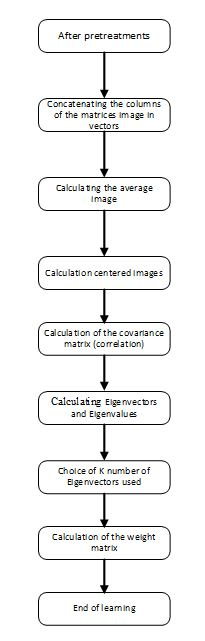
\includegraphics[scale=0.85]{ef_learningphase}%[height=70mm,width=70mm]
\caption{\textbf{EigenFaces flowchart learning phase}}%
%\url {http://www.google.fr/}
\label{ef_learningphase}%
\end {center}
\end{figure}	


\begin{figure}[bth]%[!ht]
\begin{center}
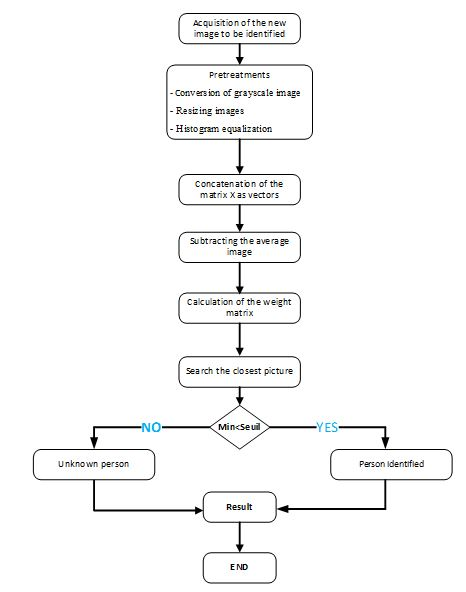
\includegraphics[scale=0.85]{ef_idphase}%[height=70mm,width=70mm]
\caption{\textbf{EigenFaces flowchart identification phase}}%
%\url {http://www.google.fr/}
\label{ef_idphase}%
\end {center}
\end{figure}	
 \newpage
\subsection{Benefits and deficiencies}	
\subsubsection{Benefits}	
Eigenface provides an easy and cheap way to realize face recognition in that:
\begin{itemize}
\item Its training process is completely automatic and easy to code. 
\item Eigenface reduces statistical complexity in face image representation.
\item Eigenface can used large databases.
\end{itemize}


\subsubsection{Deficiencies}
The deficiencies of the eigenface method are:
\begin{itemize}
\item Very sensitive to lighting, scale and translation;
\item Eigenface has difficulty capturing expression changes. 
\end{itemize}

The most significant eigenfaces are mainly about illumination encoding and don't provide useful information regarding the actual face.


%%%%%%%%%%%%%%%%%%%%%%%%%%%%%%%%%%%%%%%%%%%%%%%%%%%%%
\section{Fisherfaces}
Eigenface method uses PCA for dimensionality reduction, which yields projection directions that maximize the total scatter across all classes of images. This projection is best for reconstruction of images from a low dimensional basis. However, this method doesn’t make use of between-class scatter. The projection may not be optimal from discrimination for different classes.

While this is clearly a powerful way to represent data, it does not consider any classes and so a lot of discriminative information may be lost when throwing components away.

The Fisherface method is an enhancement of the Eigenface method that it uses Fisher’s Linear Discriminant Analysis (FLDA or LDA) for the dimensionality reduction. The LDA maximizes the ratio of between-class scatter to that of within-class scatter, therefore, it works better than PCA for purpose of discrimination. The Fisherface is especially useful when facial images have large variations in illumination and facial expression.

This projection maximizes the ratio of between-class scatter to that of within-class scatter. The idea is that it tries to “shape” the scatter in order to make it more reliable for classification.

\subsection{Linear Discriminant Analysis (LDA)}
The Linear Discriminant Analysis (LDA) is used to find the linear combination of characteristics that better separate  object or event classes. The resulting combinations can be used as a linear classifier, or generally in reducing characteristics before the posterior classification.

LDA is closely related to the PCA, because both seek the linear combinations of the variables that better represents the data. This statistic skill explicitly to model the difference between data classes unlike the PCA which does not take into account the differences between classes.
\subsection{LDA for recognition}
The LDA by recognition algorithm is divided into two phases, one for the calculation of person  models called system learning phase and the other which is to recognize a person thanks to registered models called test stage.
\subsubsection{Learning phase}
As in the PCA, it gathers the images of the learning database in a large image matrix T where each column represents a image listed Ti, then the average image is calculated.
For each class C, the average image is calculated.
Each image Ti of each class Ci is then refocused in comparison of the average. This produces a new image.
Then we proceed at calculation of the different scatter (dispersion) matrixes named as followed:
\begin{itemize}
 

\item The Intra-class Distribution Matrix;
\item The Inter-class Distribution Matrix;
\item Total Dispersion Matrix.
\end{itemize}
After we have defined the different dispersion matrixes, we must find the best projection that maximizes the intra-class dispersion on its matrix while minimizing inter-class dispersion, also on its matrix.

\clearpage
\begin{figure}[bth]%[!ht]
\begin{center}
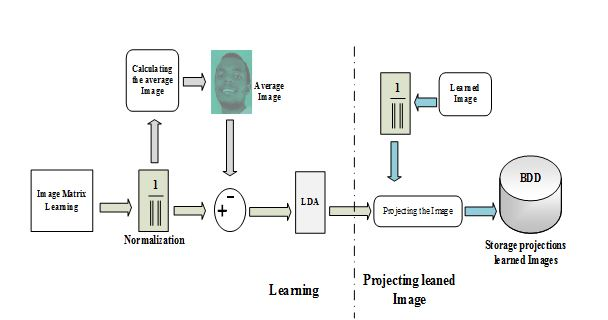
\includegraphics[scale=0.75]{learningPhaseGM}%[height=70mm,width=70mm]
\caption{\textbf{Learning phase of a face recognition system using a global method}}%
%\url {http://www.google.fr/}
\label{learningPhaseGM}%
\end {center}
\end{figure}
\subsubsection{Test phase or test stage}
Once the optimal projection that maximizes the found intraclass dispersion, the same pattern as the PCA on the projection of learned image and the projection of a test image is applied.
Then we project the test image in the Fisher space.
We compare the models obtained in learning phase. The comparison is made by calculating the distances (for instance, one can use calculation of the Euclidean Distance) between models and the test vectors and a decision rule is used to classify people.
\begin{figure}[bth]%[!ht]
\begin{center}
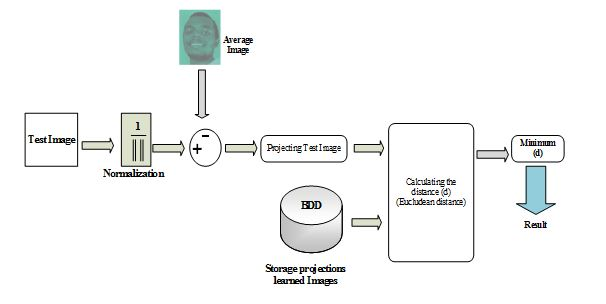
\includegraphics[scale=0.75]{TestphaseGM}%[height=70mm,width=70mm]
\caption{\textbf{Test phase of a face recognition system using a global method}}%
%\url {http://www.google.fr/}
\label{TestphaseGM}%
\end {center}
\end{figure}
\newpage
\subsection{Fisherfaces flowchart }
\begin{figure}[bth]%[!ht]
\begin{center}
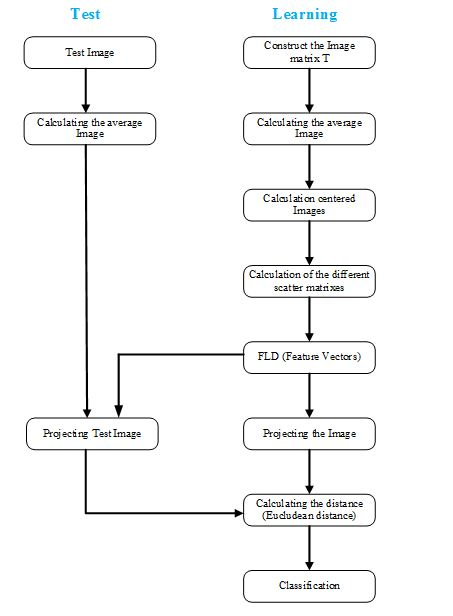
\includegraphics[scale=0.85]{test_learn}%[height=70mm,width=70mm]
\caption{\textbf{FisherFaces flowchart}}%
%\url {http://www.google.fr/}
\label{test_learn}%
\end {center}
\end{figure}

\subsection{Benefits and deficiencies}
The use of the LDA method for face recognition afford the following advantages:
\begin{itemize}
\item Maximizing inter-class scatter ;
\item Reduction of intra-class scatter ;
\item The method of Fisherfaces solves the problem of robustness to changes in pose, and facial expressions.
\end{itemize}

Despite these advantages, in the literature a serie of negative spikes still exists as:
\begin{itemize}
\item Costly (heavy) in computation time ;
\item Costly (heavy)  in memory space ;
\item Makes poor results when the number of training images is great.
\end{itemize} 


















 
 
 














































 
 
 
 
 
 
 
 
 



